\documentclass[12pt]{article}
\usepackage[a4paper, left=2cm, right=2cm, top=2cm, bottom=2cm]{geometry}
\usepackage[utf8]{inputenc}
\usepackage[T1]{fontenc}
\usepackage[french]{babel}
\usepackage{graphicx}
\usepackage{lmodern}
\usepackage{minted}
\usepackage{csquotes}
\usepackage{xcolor}
\usepackage{color}
\usepackage[backend=biber,style=numeric,sorting=none]{biblatex}
\usepackage[xindy]{glossaries}
\usepackage[hidelinks]{hyperref}
%\graphicspath{ {images/} }

\parskip=5pt plus2pt minus 1pt
\frenchbsetup{ReduceListSpacing=false}

\definecolor{back}{HTML}{ebebe0}

%\catcode`\|=13
%\def|#1|{\texttt{\detokenize{#1}}}

\addbibresource{bibli.bib}
\makeglossaries

\title{\gls{PdP} \smallbreak Mémoire }
\author{Lorian Corbel \\ Camille Meyrignac \\ Maxime Pacaud \\ Nicolas Sentout}

\begin{document}

% ACRONYMS HERE
\newacronym{PdP}{PdP}{Projet de Programmation}
\newacronym{GPU}{GPU}{Graphics Processing Unit}
\newacronym{GLSL}{GLSL}{OpenGL Shading Language}
\newacronym{VBO}{VBO}{Vertex Buffer Object}
\newacronym{IBO}{IBO}{Index Buffer Object}
\newacronym{VAO}{VAO}{Vertex Array Object}

% DEFINITIONS HERE
\newglossaryentry{marque}
{
    name=marque,
    description={Les marques sont les éléments basiques, c'est à dire des formes primitives dont les
    propriétés peuvent être gérées par des données liées}
}
\newglossaryentry{canaux}
{
    name=canaux,
    description={Caractéristique d'une marque; ex: position, taille, rotation, profondeur, couleur, etc}
}
\newglossaryentry{crate}
{
    name=crate,
    description={Une crate est une collection de code source Rust}
}
\newglossaryentry{shader}
{
    name=shader,
    description={Programme GLSL}
}
\newglossaryentry{vertex}
{
    name=vertex,
    description={Point d'informations graphiques}
}
\newglossaryentry{uniform}
{
    name=uniform,
    description={Un uniform est une variable globale GLSL}
}
\newglossaryentry{pipeline}
{
    name=pipeline,
    description={Succession des opérations généralement réalisées par une carte graphique nécessaires au
    rendu d'un lot de données}
}
\newglossaryentry{geom}
{
    name={geometry shader},
    description={Un programme shader écrit en GLSL qui régit le traitement des primitives (marque)}
}

\newglossaryentry{frag}
{
    name={fragment},
    description={Un ensemble d'information destiné à devenir un pixel}
}


\newglossaryentry{unsafe}
{
    name={unsafe},
    description={Partie de code qui ne garantit pas la sécurité de mémoire promis par Rust}
}

\maketitle
\tableofcontents
\newpage

\section{Abstract}

De nos jours le Big Data demande de créer des bibliothèques de visualisation de données pouvant afficher plusieurs centaines de milliers de visuels tant en maintenant un nombre d'image par seconde satisfaisant.
C'est dans ce contexte que Romain Giot a proposé de réaliser un moteur de rendu en Rust gérant les animations et dont la performance est l'objectif principal. Nous avons réalisé une bibliothèque pouvant manipuler plusieurs types de formes, supportant les animations et dont les performances sont supérieurs à celles de bibliothèques similaires.


\section{Travaux précédents}

Nous nous sommes basés sur deux bibliothèques afin de réaliser ce projet.
Premièrement la bibliothèque FATuM, une bibliothèque C++ qui se veux être un compromis entre le heut et le bas niveau, la bibliothèques donne la possibilité d'autres bibliothèques dont l'interface serait plus adapté pour une utilisation de haut niveau sans avoir à ce soucier de la vitesse de rendu.

La seconde bibliothèques, vega écrite en javascript est une bibliothèque visant à donner divers outils de dessin pour des bibliothèques de plus haut niveau.

Finalement notre client nous a aussi donner un proof of concept de ce que nous devions implémenter. Écrite en Rust, cette bibliothèque propose l'affichage de plusieurs type de forme que nous devions nous aussi être capable d'afficher.

\section{Analyse des besoins}
%% Etoffer la partie analyse des besoins
\subsection{Analyse des besoins fonctionnels}

L'utilisateur doit être capable d'appeler des fonctions de la bibliothèque permettant d'afficher des
\gls{marque}s \cite{VegaMarks}. Les divers types de marque sont les suivants:
	\begin{itemize}
	\item Points : utilisable pour faire des nuages de points. La forme des points dépend d'une fonction de
    distance calculée en GLSL. Nous reprendrons les mêmes marques que celles du proof of concept de notre client.
    Ainsi les marques à implémenter seront: Rectangle, Triangle, Cercle, Point,Diamant, Donut, Pointeur (pointeur de carte ou de gps), Trèfle, Cœur, 			Pique, Chevron, Trèfle à trois feuilles (recoupement de trois cercles), Anneau, Dièse, Croix, Astérisque, Infini, Flèche. 
    \item Lignes : utilisable tel quel ou pour faire des connexions entre d'autres marques. Les lignes
    peuvent être des segments, des polylignes ou des courbes, elles peuvent aussi avoir différents types
    (continu, tirets, pointillés...). 
    \item Polygones : utilisable pour représenter des polygones pleins ou vides, où l'on appelle vide un 
    polygone dont seulement les contours sont dessinés, la couleur de remplissage du polygone plein peut être
    différente de la couleur des contours. 
    \item Aires : utilisable pour représenter des polygones ayant un mode d'affichage légèrement différent
    \cite{VegaMarks}. Ces aires doivent permettre à l'utilisateur de représenter des aires sous la courbe lorsqu'il fait de la
    visualisation de données. Ces types de marque ne sont pas le plus prioritaire à implémenter.
    \item Texte : utilisable pour représenter du texte et peut avoir différentes propriétés : italique,
    gras, centré, aligné à droite, en haut, etc.
    \end{itemize}
\begin{itemize}
\item L'utilisateur doit notamment être capable de préciser des \gls{canaux} associés à
ces marques : la position de la marque, sa taille, sa rotation, sa profondeur, sa couleur, sa forme,
l'épaisseur et la couleur de son contour, son contraste, sa luminance, son rayon, ses angles, etc.
\item \textit{Contrast} devra également être capable de gérer des calques, c'est-à-dire que l'utilisateur pourra
décider de placer une marque sur un certain calque et une autre marque sur un différent calque. Si ces
marques ont la même position, l'une des deux marques cachera la seconde. Cet exemple utilise deux calques
mais il peut y en avoir autant que l'utilisateur le souhaite.
\item Une caméra simple pour visualiser la scène en 2D doit être implémentée. À priori, elle ne fait pas
de translation, le seul paramètre qu'elle prend en compte est un niveau de zoom ainsi que la taille
de la fenêtre d'affichage.
\item La bibliothèque devra être implémenté de deux façons différentes. Un implémentation bas-niveau et une implémentation haut-niveau. 
Le bas-niveau permettra à l'utilisateur d'implémenter le moteur de rendu comme il le souhaite afin de gérer le contexte OpenGL, en haut-niveau
nous fournissons le moteur de rendu.
		\begin{itemize}
			\item Pour simplifier le rendu en OpenGL nous utiliserons \textit{luminance} \cite{luminance}, nous avons choisi cette bibliothèque
			premièrement elle nous a été proposé par notre client et de plus c'est une des seules bibliothèque de rendu OpenGL sur Rust et celle-ci est
			très souvent mise à jour.
			\item En haut-niveau nous aurons aussi besoin de gérer les événements clavier.
		\end{itemize}
\item Les marques devront être animées de façon similaire à FATuM.
	\begin{itemize}
	\item Pour ce faire nous utiliserons un double tampon pour la visualisation, un tampon servant de tampon avant et un tampon servant de tampon arrière.
	Le tampon avant est utilisé pour l'affichage et le tampon arrière est utilisé pour les modifications de l'image affichée et quand l'opération de mise
	à jour est finie (c'est-à dire que l'on a une autre image à afficher).
	\item Les deux tampons peuvent être échangés par différentes techniques notamment un simple échange : le tampon arrière devient le tampon avant et
	inversement, ou on peut utiliser une interpolation progressive des deux images stockées dans les tampons. De ce fait, l'image affichée n'est changée
	que quand il y a une autre image prête, ce qui évite le problème de l'affichage se mettant à jour petit à petit, donnant lieu à des animations peu
	lisible.
	\item Un troisième tampon peut être utilisé pour empêcher l'annulation d'une animation si l'utilisateur demande une modification pendant une
	animation. Le troisième tampon stocke les modifications faites par l'utilisateur durant l'animation et seront utilisées pour la prochaine animation.
	\end{itemize}
\end{itemize}  



\subsection{Analyse des besoins non fonctionnels}

L'objectif principal de ce projet est avant tout les performances.Le but est de dépasser les performances de la bibliothèque FATuM.Pour garantir
ce besoin plusieurs choix ont été fait:
	\begin{itemize}
		\item Le client nous a demandé de réaliser le projet avec le langage Rust \cite{rust}, l'intérêt de ce langage est qu'il offre de très bonnes
		performances pour l'application, comparable à du C mais aussi un système de sécurité de la gestion de mémoire,permettant de garantir un programme
		sans fuite mémoire ni erreur de segmentation.
		\begin{itemize}
			\item Nous serons obligés de réaliser du code \gls{unsafe} pour cette bibliothèques mais l'objectif et d'en faire le moins possible.
			\begin{itemize}
				\item Il faudra donc mettre en place une batterie de tests importante pour ces parties particulièrement sensibles.
			\end{itemize}
			\item Nos devrons écrire des macros afin d'éviter les doublons dans le code.
		\end{itemize}
		\item Le client nous demande aussi de réaliser la partie GPU à l'aide d'OpenGL. Le but est de réaliser le maximum des algorithmes de génération de 		nos marques sur GPU et donc en OpenGL afin d'épargner un maximum de calcul au processeur.
		\begin{itemize}
			\item Nous devrons utiliser un \gls{geom} en glsl pour les marques afin de limiter le nombre de vertices passées au GPU.
			\item Il faudra séparer les \gls{shader}s de chaque type de marque dans plusieurs fichiers différents.
			\item Notre client souhaite que nous utilisons une crate Rust pour compiler
			nos shaders en GLSL, afin de construire et nous assurer de leur bonne conformité.
			La crate en question porte le même nom que GLSL\cite{GLSL}.
		\end{itemize}
		\item Des benchmark devront être réaliser pour comparer les performances de notre programme aux logiciels déjà existant, principalement FATuM.
	
	\end{itemize}
Le niveau de priorité de chaque besoin est le suivant :
\begin{itemize}
	\item Marque Point
	\item Marque Ligne
	\item Calques
	\item Animations
	\item Marque Texte
	\item Marque Polygone
	\item Marque Aire
\end{itemize}

Pour l'API l'utilisateur devra décrire les divers propriété de chaque marque de la façon suivante:
\begin{itemize}
    \item Pour les marques point :
    
    \begin{minted}[bgcolor=back, tabsize=4, fontfamily=courier, fontsize=\small, xleftmargin=5pt, xrightmargin=5pt]{rust}
    contrast.add_point_mark().set_position(100.0,50.0,0.0).set_size(size)
    .set_color(1.0,1.0,0.0,0.0).set_shape(Spade);
    \end{minted}
    
    \item Pour les marques ligne il faudra pouvoir préciser plusieurs points pour les polylignes :
    \begin{minted}[bgcolor=back, tabsize=4, fontfamily=courier, fontsize=\small, xleftmargin=5pt, xrightmargin=5pt]{rust}
    contrast.add_line_mark().add_point(pos)
        .add_point((50.0,50.0,0.0))
        .add_point(pos2)
        .set_thickness(20.0)
        .set_color((1.0, 0.0, 0.0, 1.0))
        .get_id();
    \end{minted}
    \item Pour les marques texte il faut avant charger des font dans \textit{Contrast} puis les utiliser :
     \begin{minted}[bgcolor=back, tabsize=4, fontfamily=courier, fontsize=\small, xleftmargin=5pt, xrightmargin=5pt]{rust}
     contrast.register_font("helvetica", helvetica_font_file, 120);
     contrast.add_text_mark()
        .set_position((30.0, 300.0, 1.0))
        .set_font("helvetica")
        .set_text("White")
        .set_color((1.0, 1.0, 1.0, 1.0));
    \end{minted}
    \item Voici maintenant un exemple d'utilisation des calques :
    \begin{minted}[bgcolor=back, tabsize=4, fontfamily=courier, fontsize=\small, xleftmargin=5pt, xrightmargin=5pt]{rust}
     // On créer un marque m
     
     contrast.add_layers(2);
     let layer_0=contrast.get_layer(0);
     layer_0.add_mark(m);
    \end{minted}
    \item Pour la gestion du clavier on aura deux fonction, une qui permet une action sur une marque spécifique, une autre qui le permet sur un ensemble 
    de marques :
    \begin{minted}[bgcolor=back, tabsize=4, fontfamily=courier, fontsize=\small, xleftmargin=5pt, xrightmargin=5pt]{rust}
    // m1 est une marque
    renderer.add_mark_action_on_press(Key::Space, action1, m1);
    // marks est un vecteur de plusieurs marques 
    renderer.(Key::F, action2, marks);
    \end{minted}
    \item Il faut aussi notifier à contrast de se mettre à jour lorsque de nouvelles marques sont ajoutés, pour cela nous utiliserons :
    \begin{minted}[bgcolor=back, tabsize=4, fontfamily=courier, fontsize=\small, xleftmargin=5pt, xrightmargin=5pt]{rust}
    contrast.mark_dirty_all();
    \end{minted}
    \item En haut-niveau il faudra initialiser notre moteur de rendu :
    \begin{minted}[bgcolor=back, tabsize=4, fontfamily=courier, fontsize=\small, xleftmargin=5pt, xrightmargin=5pt]{rust}
    let mut renderer = LumiRenderer::init(WINDOW_WIDTH, WINDOW_HEIGHT, "Titre");
    \end{minted}
    \item Il faudra aussi récupérer le contrast du renderer et l'initialiser de la façon suivante :
    \begin{minted}[bgcolor=back, tabsize=4, fontfamily=courier, fontsize=\small, xleftmargin=5pt, xrightmargin=5pt]{rust}
    let contrast = renderer.get_contrast_mut();
    \end{minted}
    \item Toujours en haut-niveau il faudra lancer une boucle de rendu avec 
    \begin{minted}[bgcolor=back, tabsize=4, fontfamily=courier, fontsize=\small, xleftmargin=5pt, xrightmargin=5pt]{rust}
    renderer.run();
    \end{minted}
    
\end{itemize}
\section{Description du logiciel}
%% Parler des problèmes rencontrés au sain de l'archi
\subsection{Organisation de l'architecture}

Notre bibliothèque est composée de 2 parties principales :
\begin{itemize}
\item la partie bas niveau, contenu dans le dossier \textit{contrast}
\item la partie haut niveau, contenu dans le dossier  \textit{contrast-renderer}.
\end{itemize}

La partie bas niveau est elle-même séparée en plusieurs dossiers ;
\begin{itemize}
\item \textit{mark\_macro\_derive}, qui contient l'implémentation de la macro procédurale
\item \textit{properties}, qui contient l'implémentation de plusieurs propriétés utilisées par la bibliothèque
\item \textit{src}, le code source principal de la partie bas niveau, contenant l'implémentation des structures de données pour stocker les marques, la structure principale gérant les marques et les shaders pour tous les types de marques.
\end{itemize}

\subsection{Architecture bas niveau}

L'architecture bas niveau est composée d'une structure principale contenant tous les calques. Les calques contiennent
chacun leurs marques.

La figure~\ref{fig:arch} décrit de manière simplifiée l'architecture.

\begin{figure}[htp]
  \centering
  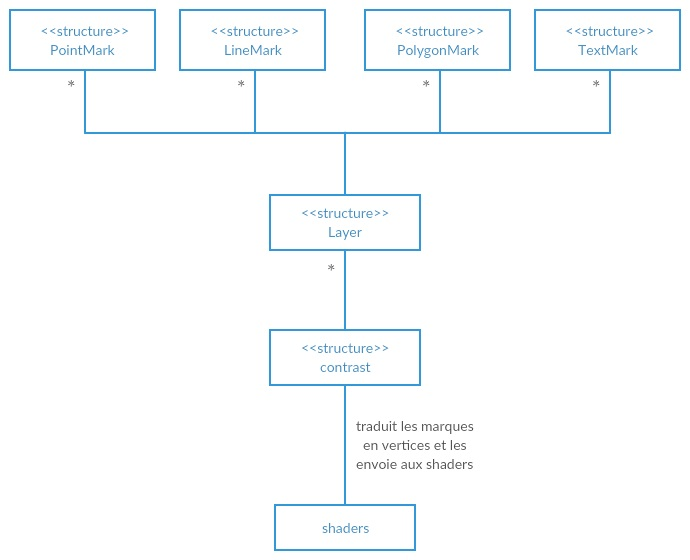
\includegraphics[scale=1.0]{images/architecture}
  \caption{Diagramme simplifié de l'architecture de \textit{contrast} }
  \label{fig:arch}
\end{figure}

\textit{Contrast} supporte différents types de marques mais elles ont en commun certaines propriétés.
Elles ont toutes une identifiant, font parties d'un calque et ont une couleur.
La solution venant directement à l'esprit pour représenter de telles structures est celle de l'héritage.
Toutes nos marques hériteraient d'une structure qui contient ces propriétés communes ainsi que certaines
méthodes communes.
Cependant, Rust ne supporte pas l'héritage. Nous devons donc utiliser des solutions propres à Rust pour régler
ce problème.
Nous avons donc utilisé une macro procédurale. C'est une macro permettant de générer du code à la
compilation. Elle permet de fournir une implémentation par défaut à un trait. Nos structures peuvent
ensuite dériver de ce trait. Elles auront ainsi accès aux méthodes implémentées par la macro.

Toujours pour palier à ce problème d'héritage, nous disposons d'une union de toutes les structures
de données des marques. Cela permet de stocker nos marques plus facilement et d'utiliser des conteneurs d'union plutôt que des conteneurs pour chaque type de marque.

Côté GLSL, nous disposons de shaders différents pour chaque type de marque. Toutes nos marques utilisent un vertex shader, un \gls{geom} et un \gls{frag} shader à l'exception du texte qui n'utilise pas de geometry shader.

\subsection{Pipeline graphique}

Le pipeline graphique est la succession des opérations généralement réalisées par une carte graphique nécessaire au rendu d’un lot de données. Nous allons essayer de vous décrire en détails comment
fonctionne celui de \textit{contrast}. Nous allons nous appuyer sur OpenGL comme exemple mais c'est quelque chose d'assez générique à toutes les API graphiques. Ce seront donc les mêmes concepts pour
Vulkan ou DirectX seulement probablement sous une autre dénomination.

OpenGL ne sait dessiner que des primitives de dessins très simples comme le point (litteralement un pixel) ou le triangle. Toute forme complexe est impossible sans traitement.
Ces primitives sont définies par des vertices, qui sont des sommets qui portent différents attributs. Nous avons par exemple deux attributs très utilisés qui sont la position et
la couleur, mais toute autre information est imaginable. Ce qui est certain, c'est qu'il faut 3 vertices pour dessiner un triangle.

En réalité les attributs d'un vertex sont des flottants ou même des tableaux de flottants. C'est ce qu'on peut appeler un vecteur. L'ensemble de ces vertices est stocké dans ce
que OpenGL appelle un \gls{VBO}, c'est-à-dire un énorme buffer présent dans la mémoire du GPU. La description des attributs d'un vertex est fait par le \gls{VAO}.
C'est lui qui va décrire combien il y a d'attributs par vertex et si ce sont des vecteurs de une à quatre dimension.
Cette description permet au shader program de pouvoir accéder à ses vecteurs et les manipuler.

Le shader program est un programme écrit en \gls{GLSL} qui est exécuté sur le GPU. Il est découpé en plusieurs passes, voici les trois essentiel dans l'ordre d'exécution :
\begin{itemize}
    \item Le vertex shader permet de définir en sortie la position du vertex sur l'écran. C'est par lui qu'arrive l'ensemble
des attributs mais ils peuvent toujours atteindre les autres étages si le vertex shader leur transmet en sortie.
    \item Le geometry shader permet d'émettre davantage de vertices qu'il en a initialement reçu du VBO. Il permet donc de modifier la géometrie de notre primitive de dessin.
    \item Le fragment shader permet de définir la couleur de sortie des pixels (appelé fragments) de notre primitive.
\end{itemize}

Pour résumer, pour afficher un triangle, une fois que notre VBO est rempli, notre VAO défini et que notre shader program écrit, il faut dire à OpenGL d'afficher la primitive.
C'est un appel \og draw \fg{} qui s'occupe de cette tâche, il prend en paramètre le type de la primitive de dessin et combien il faut en dessiner.

La quantité de primitives à dessiner est très importante. C'est une optimisation primordiale à maximiser. Il faut diminuer le plus possible la communication entre le CPU et le GPU pour
qu'au final, le GPU soit quasiment autonome et puisse sous-traiter le plus possible le travail du CPU pour que celui-ci se concentre sur des tâches plus importantes.
C'est pour cette raison qu'on essaie d'afficher le plus de primitives en seul appel : pour que le CPU n'est seulement à communiquer ses appels draw à chaque frame pour dessiner entièrement
un rendu. Cette méthode s'appelle le batching, c'est-à-dire le dessin par lot.

Ainsi la couche bas niveau de \textit{contrast} possède un shader program et un format de vertex par type de marque qui seront transmis à la couche haut niveau pour afficher les marques.
Pour rappel, c'est la partie haut niveau qui s'occupe d'OpenGL, car selon notre cahier des besoins, on doit pouvoir utiliser une autre API graphique. Les vertices que nous avons
défini dans nos shaders sont complètement génériques pour fonctionner sur une autre implémentation.

\subsection{Architecture haut niveau}

L'architecture haut niveau est chargé de ce que nous appelons le \og renderer \fg{}. Il dépend entièrement de l'API graphique que nous allons utiliser ainsi que la bibliothèque
de fenêtrage qui gère aussi les événements clavier/souris. Cette couche haut niveau contient \textit{contrast} et masque toute la partie rendu.
Nous avons implémenté un renderer avec la crate \textbf{luminance} \cite{luminance}, comme demandé par notre client dans un de ses besoins.
Luminance utilise OpenGL mais ne nous donne pas accès directement à toutes ses fonctions, il nous a fallu respecter la nomenclature et l'API de Luminance.

Notre architecture haut niveau est donc intrésequement liée à \textit{luminance}. La seule implémentation intéressante dans cette partie est comment nous avons mis à jour les VBOs que \textit{luminance} cache
en réalité derrière ce qu'elle appelle un \og Tess \fg{}. C'est en réalité un VBO + VAO.

Le tess de \textit{luminance} prend à sa création une taille fixe de vertices (la capacité du VBO). Cette taille ne peut pas être modifiée par la suite. Comment faire dans ce cas pour afficher davantage
de marques lors de l'exécution ?

Nous avons réglé le problème plutôt simplement. Il nous a suffi d'allouer un tess de grande taille, initialisé completement à zéro. Les vertices des marques à afficher sont ajoutés
progressivement dans le tess et pour afficher, nous appelons le \og draw \fg{} du batching uniquement sur la partie remplie du tess. Nous n'avons pas poussé la gestion de la mémoire très loin.
Si par exemple, on souhaite supprimer une marque, nous demandons à \textit{contrast} l'intégralité des vertices de ce type de marque et nous les recopions en tête de tableau. Reste à prendre en compte la
nouvelle taille et la mise à jour est terminée. Nous avons choisi de faire la même chose pour l'ajout, la suppresion ou simplement pour mettre à jour une marque. C'est essentiellement à cause d'un
manque de temps et par facilité d'implémentation. \textit{contrast} peut prévenir notre renderer à l'aide de flags pour savoir quel tess il doit mettre à jour.

Malheureusement, il peut arriver que la taille du tess soit dépassée. Dans ce cas nous n'avons plus le choix, le tess doit être détruit et ré-alloué en conséquence avec une dimension plus convenable.


%% TODO ce schema doit être mis à jour
\begin{figure}[htp]
  \centering
  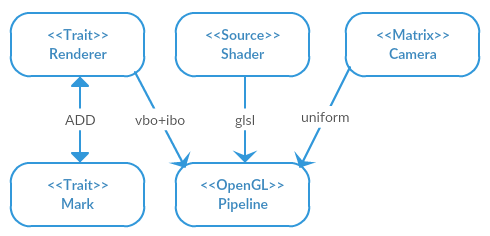
\includegraphics[scale=0.8]{images/pipeline}
  \caption{Diagramme de schématisation du pipeline}
  \label{fig:pipe}
\end{figure}

\subsection{Implémentation des marques de type point}

Nous avons utilisé trois shaders en OpenGL afin de réaliser l'implémentation de ces marques. Tout d'abord le vertex shader, il
permet de manipuler les vertices, ici nous avons un seul vertex pour chaque marque. Dans une version sans animation des marques
points il faut simplement transmettre la position, la couleur, la taille, la rotation et le type de forme au shader suivant du
pipeline graphique. Ce nouveau shader est appelé geometry shader, ce shader permet de générer des nouveaux sommets permettant
de créer des nouvelles formes.

Dans notre cas, le geometry shader permet de générer un rectangle englobant dans lequel sera contenu notre forme. Nous avons
donc crée six sommet, soit deux triangles, chacun étant une moitié de notre rectangle englobant. C'est lors de la création de
ces sommets que nous appliquons la rotation à notre forme et que nous lui appliquons une matrice de projection afin de faire
passer cette forme dans le repère de l'observateur, c'est à dire que l'affichage de cette forme dépend maintenant de la caméra.
On doit ensuite passer à l'étape où la forme à proprement parler est calculée.

Ainsi, nous arrivons ensuite dans le dernier shader, le fragment shader, le principe de ce shader est de calculer la couleur
finale de chaque pixel qui est affiché à l'écran. Dans ce shader, on utilise une fonction de distance entre le \gls{frag} en
cours de traitement et le centre de notre rectangle englobant afin de savoir si chaque pixel de ce rectangle fait parti ou non
de la forme souhaitée. Les fonctions de distance utilisées sont tirées du papier de Nicolas Rougier \cite{Rougier}. On calcule
cette fonction distance différemment pour chaque forme, puis si la distance est trop grande, on se défausse du \gls{frag}. On
génère donc notre forme de manière procédurale.

Cette implémentation à été choisie car elle nous permet de n'avoir besoin que d'un seul sommet pour réaliser des formes complexes.
Tous les traitements sont réalisés coté GPU, ce qui permet un énorme gain de performances par rapport à une implémentation où
l'on devrait fournir tous les sommets de notre forme avant de devoir l'afficher. C'est un gain particulièrement important pour
des formes arrondies nécessitant beaucoup de sommets pour éviter l'aliasing.
L'avantage du fragment shader est aussi que chaque \gls{frag} est traité de manière indépendant, il y a donc une très forte
parallélisation des traitements au sein du fragment shader, parallélisation qui est la grande force des GPU.

On retrouve toutes les formes pouvant être générées par nos shaders des marques point dans la figure~\ref{fig:point-marks}.
\begin{figure}[htp]
  \centering
  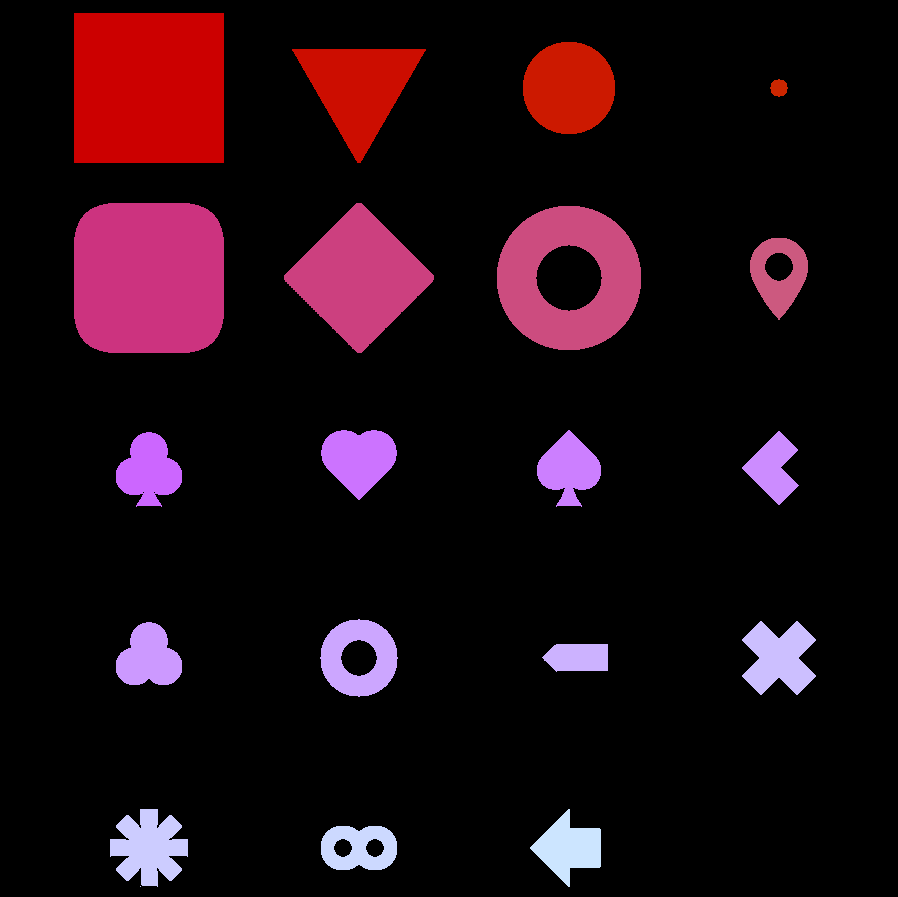
\includegraphics[scale=0.5]{images/point_mark}
  \caption{Affichage de toutes les marques de type point}
  \label{fig:point-marks}
\end{figure}

\subsection{Implémentation des marques de type ligne}
\subsubsection{Les shaders utilisés}
Pour cette marque, nous avons utilisé trois types de shaders OpenGL, qui sont les mêmes que ceux de la rubrique précédente.

<<<<<<< HEAD
Pour l’implémentation de cette marque le vertex shader sert seulement à envoyer
 les données vers le geometry shader, de ce fait il y a peu à dire sur ce shader.
 Le vertex shader reçoit donc et envoie donc les données utiles pour l’affichage
 d’une sous ligne de la polyligne, de fait il reçoit comme information la position
 d’origine et de fin de la sous-ligne en question et de plus il reçoit les informations
 de position du point précédent la sous-ligne et celle du point suivant la sous-ligne
 (nous expliquerons plus en détail pourquoi nous avons besoins de ces informations).
 Le fragment shader sert exclusivement à appliquer la couleur de la ligne sur les fragments.
=======
Le vertex shader sert seulement à envoyer les données vers le geometry shader. De ce fait, il y a peu à dire sur ce shader.
Le vertex shader reçoit et envoie donc les données utiles pour l’affichage
d’une sous ligne de la polyligne, de fait elle reçoit comme information la position
d’origine et de fin de la sous-ligne en question. De plus, elle reçoit les informations
de position du point précédent de la sous-ligne et celle du point suivant la sous-ligne
(nous expliquerons plus en détail pourquoi nous avons besoins de ces informations).
Le fragment shader sert exclusivement à appliquer la couleur de la ligne sur les fragments.
>>>>>>> 33a55a547aedbbed4dd12e320810e25452c4d4bc

Pour afficher une ligne à largeur variable nous avons deux possibilités :
\begin{itemize}
\item soit utiliser la primitive OpenGL \og GL\_LINES \fg{}, ce qui demanderait un nombre de primitives dépendants de la largeur de la ligne, ce qui ne serait pas très efficace
\item soit utiliser une des primitives OpenGL servant à afficher des triangles comme par exemple \og GL\_TRIANGLE\_STRIP \fg{} pour afficher le quadrilatère (donc avec quatre sommets) correspondant à une sous-ligne, dont le nombre de primitives utilisés ne dépend pas en complexité de la taille ou de la largeur de la ligne.
\end{itemize}

Nous avons utilisé la deuxième possibilité, qui semble meilleure en terme de performance.
Considérant le fait qu’il faille diminuer au maximum le coût du calcul côté GPU, les quatre sommets du quadrilatère seront
calculés sur le GPU et donc avec l’unique shader capable de faire ce genre d’opératio­n, c’est-à-dire le geometry shader, avec
la primitive \og GL\_TRIANGLE\_STRIP \fg{}.

\subsubsection{Liaison entre les sous-lignes}
Simplement afficher des rectangles représentant les sous-lignes est possible pour une polyligne formée de seulement deux points. Mais pour plus de points, il faut gérer la liaison entre les sous-lignes, sinon nous aurons une jonction entre les deux sous-lignes peu attrayante. Il y a plusieurs façon de faire pour gérer cette liaison, comme le montre la figure~\ref{fig:joint}.

\begin{figure}[htp]
  \centering
  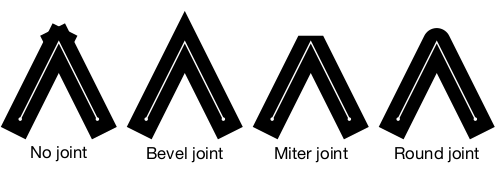
\includegraphics[scale=0.8]{images/line-joints}
  \caption{Schéma de la géométrie de la ligne}
  \label{fig:joint}
\end{figure}

La solution la plus simple en terme de performances se trouve être le \og bevel join \fg{}, étant donné que cette liaison peut-être réalisée juste en changeant l’inclinaison du bout de chaque sous-ligne. On garde ainsi le fait de n’avoir à afficher qu’un
quadritère par sous-ligne alors que la solution de la liaison  \og round joint \fg{} n’est pas aussi simple et demande de
retirer des pixels au bord d’un quadrilatère un peu de la façon de l’implémentation de la marque point (de plus utiliser la
fonction discard d’OpenGL dans le fragment shader diminue les performances pour la plupart des hardwares\cite{FragmentDiscard}).

Pour faire la liaison choisie, il nous faut le voisinage des points formant une sous-ligne de façon à avoir une inclinaison des
extrémités de sous-ligne s’accordant. Pour expliquer plus facilement comment est formée cette liaison voici la figure~\ref{fig:geom_line}.

\begin{figure}[htp]
  \centering
  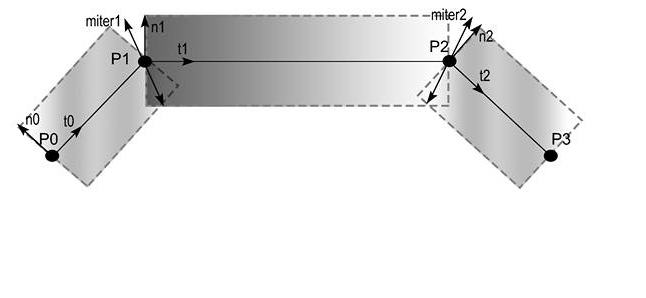
\includegraphics[scale=0.8]{images/line_geom}
  \caption{Schéma de la géométrie de la ligne}
  \label{fig:geom_line}
\end{figure}

Dans ce schéma, les vecteurs miter1 et miter2 sont ce que j’appelle précédemment l’inclinaison des extrémités. Les vecteurs t0,
t1, et t2 sont respectivement les vecteurs directeurs des segments [P0,P1], [P1,P2], [P2,P3] et n1, n2 et n3 leurs normales. De
ce fait, le miter n’est en fait que l’addition des vecteurs normaux des segments correspondants. Il faut aussi calculer la
valeur d’écart par rapport au point d’origine pour avoir une ligne avec une largeur correcte. Pour cela, on prend la largeur
voulue de la ligne et on le divise par le produit scalaire de la normale de la ligne précédente ou suivante suivant l’extrémité et le miter correspondant. Une fois que l’on a le miter, il suffit de créer des points décalés de la valeur précédemment créé le long du vecteur miter normalisé.

\subsubsection{Résultat}
Et finalement voici le résultat figure~\ref{fig:line}.
\begin{figure}[htp]
  \centering
  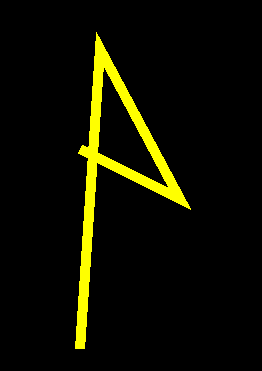
\includegraphics[scale=0.8]{images/line_example}
  \caption{Exemple d'affichage de ligne}
  \label{fig:line}
\end{figure}



\subsection{Implémentation des marques polygone}

Un polygone est défini par une liste de points relié cycliquement par des segments,
nous avons choisi de définir le polygone voulu par l'utilisateur comme étant la suite
ordonnée en fonction du temps par l'utilisateur.

\subsubsection{Un problème compliqué}
Il y a néanmoins plusieurs type de polygone qui ne sont pas forcément affiché de la même manière,
en effet un polygone peut être auto-sécant ou non, convexe
(c'est à dire que pour tout couple de points sur le contour, le segment les reliants est contenu dans le polygone),
concave c'est-à-dire non convexe.
OpenGL permet surtout d'afficher des triangles et la décomposition en triangle d'un polygone semble
une étape obligatoire. Ce qui pose problème c'est qu'il n'y a pas en Rust une bibliothèque implémentant
des algorithmes de triangulation vraiment efficace à l'image de ce que propose triangle \cite{Triangle} pour le
C++ par exemple, certaines crates implémentant ce genre d'opérations ne sont plus à jour depuis longtemps
et ne peuvent plus être utilisée correctement comme par exemple \cite{rtriangulate}. De plus il y a dans notre projet,
une obligation à diminuer au maximum le calcul côté CPU, le problème c'est que pour faire les opérations
permettant la triangulation d'un polygone, il faut tout le contexte du polygone ce qui n'est pas possible
côté GPU (on traite un nombre de vertex limité à chaque fois) et de plus on ne pourrait pas se permettre
d'implémenter des algorithmes avec une complexité trop forte comme par exemple la méthode des oreilles \cite{earClipping} qui est de plus un algorithme sous optimal. Il y a aussi la question de l'implémentation
des animations qui se pose, en effet comment gérer efficacement des animations lorsque les triangles
formant le polygone sont en nombre non défini même pour un même nombre de points formant le polygone
(par exemple avec une décomposition en chaîne monotone).
Après de long tatonnement nous avons déduit qu'il serait plus simple de gérer qu'une définition restrainte
des polygones, c'est-à-dire les polygones convexe pouvant être facilement découpé en triangle.

\subsubsection{Une triangulation pas convaincante}
Le plus simple pour trianguler un polygone convexe c'est de prendre un point de ce polygone et de former
tout les triangles contenant celui-ci avec les autres points du polygone comme le montre le schéma ~\ref{fig:triang_poly_conv}.

\begin{figure}[htp]
  \centering
  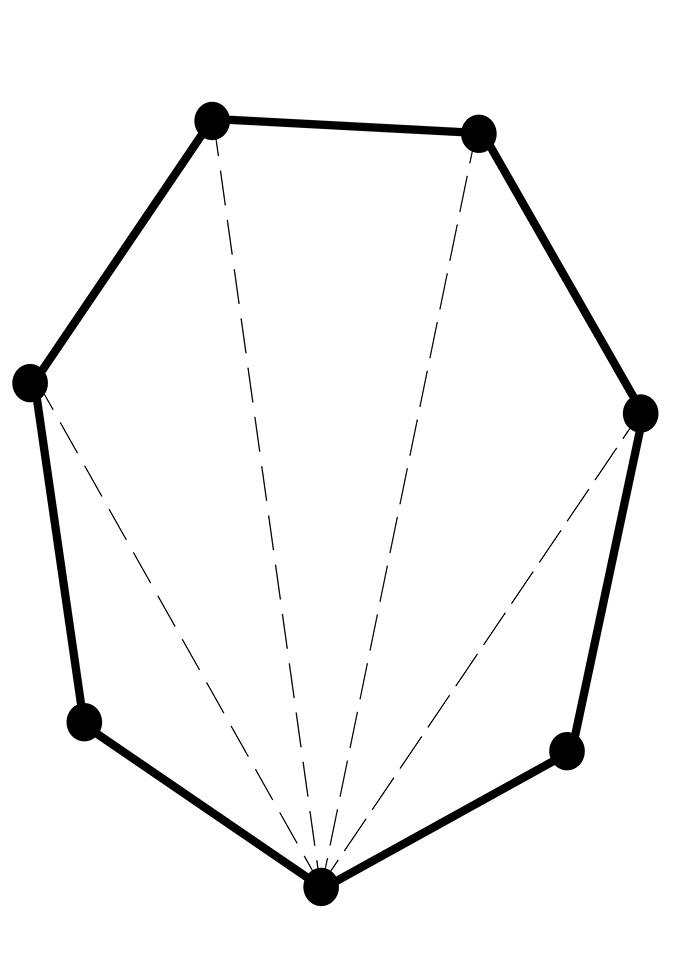
\includegraphics[scale=0.2]{images/simple_triangulation_polygon}
  \caption{Exemple de triangulation simple d'un polygone convexe}
  \label{fig:triang_poly_conv}
\end{figure}

Le gros problème de cette triangulation c'est qu'elle ne permet pas de gérer les règles de remplissage,
c'est-à-dire si l'on veut que le polygone soit rempli ou pas. Il faudrait pour ça retirer des fragments
des triangles et comme dit dans la partie sur l'implémentation de la ligne ce n'est pas optimal.

\subsubsection{Utilisation du concept de ligne}
Pour gérer les contours il faut savoir où est le centre pour ne pas agrandir l'intérieur du polygone
mais aller vers l'intérieur. Pour cela on calcule la moyenne de tout les points du polygone, ce qui
correspond en géometrie au centre de masse.
De cette manière nous pouvons former des lignes comme dans la partie sur les marques lignes mais contrairement à celle-ci nous ne centrons pas la ligne sur le point. De cette manière nous n'avons pas
de beaucoup de calcul à faire sur le CPU (le calcul du centre de masse se faisant en 0(n)) et nous pouvons
choisir la largeur du contour facilement.

\subsubsection{Résultat}

Nous pouvons voir sur ce schéma ~\ref{fig:capture_polygon_non_fill}, en haut à gauche, deux polygones définis par les mêmes points mais dont le z du polygone ayant la largeur de contour la moins épaisse est la plus haute.
En haut à droite on peut voir un polygone auto-sécant qui n'est pas affiché correctement.
En bas à gauche, un carré affiché correctement. Et finalement en bas à droite un polygone non convexe et donc affiché de manière non correcte.

\begin{figure}[htp]
  \centering
  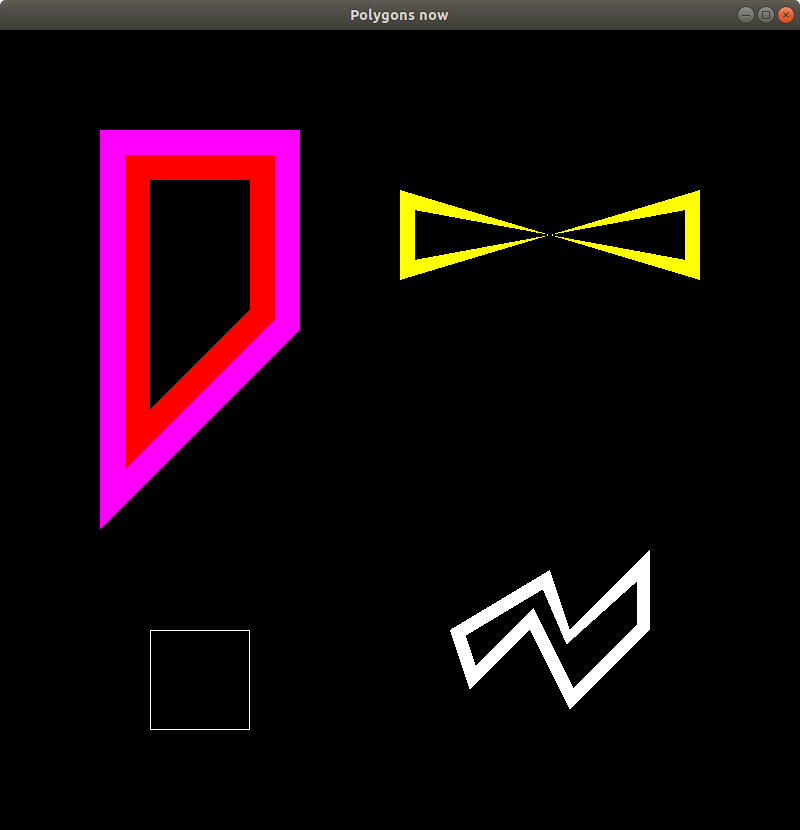
\includegraphics[scale=0.5]{images/polygon_capture}
  \caption{Exemple d'affichage de polygones vides}
  \label{fig:capture_polygon_non_fill}
\end{figure}


Nous pouvons voir sur ce schéma ~\ref{fig:capture_polygon_fill} les deux polygones correct précédent mais cette fois si remplis.
\begin{figure}[htp]
  \centering
  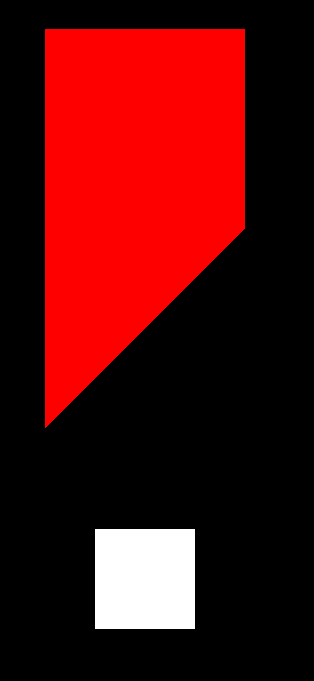
\includegraphics[scale=0.5]{images/polygon_fill}
  \caption{Exemple d'affichage de polygones remplis}
  \label{fig:capture_polygon_fill}
\end{figure}





\subsection{Implémentation des marques texte}

Un texte est une marque qui permet d'afficher une chaîne de caractère dont le contenu, la police, la taille de police ainsi que la position et couleur sont définis par l'utilisateur.

\subsubsection{Généralité}

Pour afficher du texte en fonction d'une véritable font (police), généralement vectorielle, il faut avant toute chose rastériser les caractères utilisés en bitmap.
C'est une opération complexe et c'est pourquoi nous utilisons la bibliothèque \textbf{FreeType} \cite{freetype-rs}, spécialisée dans cette fonction.

FreeType va prendre en entrée un fichier de font et la taille de police qui correspond en réalité à la hauteur en pixel d'un caractère. La largeur est calculée automatiquement
par la bibliothèque pour respecter la proportionnalité. En sortie, nous obtenons ce que FreeType appelle une \og font face\fg{} qui est propre à notre configuration font et police.
À partir de cette face, nous allons pouvoir charger chaque caractère que nous allons utiliser un par un. Il ne sont pas tous chargés car cela pourrait gâcher de la mémoire.

Un caractère rastérisé donne un glyphe. C'est une représentation graphique d'un signe typographique. Pour FreeType, c'est aussi une structure contenant toutes les métriques
du glyphe ainsi que le bitmap associé : c'est évidemment un format binaire car la couleur ne dépend pas de la font.

Une fois que nous avons rastérisé chacun des caractères de notre chaîne de caractères, nous pouvons transformer les bitmaps en texture OpenGL pour ensuite les plaquer
sur des rectangles alignés bout à bout afin de construire une chaîne de caractères lisible. Ces rectangles sont les boîtes englobantes de chaque glyphe qui dépendent
de leur métriques qui eux même sont calculées grâce à la police.
Notez que nous parlons de glyphe car ils sont forcément associés à une taille de police ainsi qu'à une font alors que ce n'est pas le cas pour un caractère.
La métrique d'un glyphe \cite{metrics} contient entre autre la hauteur et largeur du bitmap, et d'autres informations nécessaire à son bon placement pour former un mot typographiquement correct.
C'est le cas par example du \textit{bearingY} qui sert à positionner la hampe du caractère ou encore d'\textit{advance} qui est l'espacement, que l'on peut voir sur la figure~\ref{fig:metrics}.

\begin{figure}[htp]
  \centering
  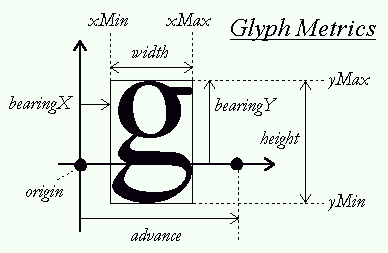
\includegraphics[scale=0.8]{images/metrics}
  \caption{Métrique de glyphe}
  \label{fig:metrics}
\end{figure}

Pour des raisons d'optimisations, nous ne pouvons malheureusement pas créer de textures par bitmap. Le moyen le plus simple d'optimiser un rendu en OpenGL et de faire du dessin par lot,
c'est-à-dire du batching. Nous reviendrons probablement dessus dans la section dédiée à la couche haut-niveau mais pour résumer brièvement, c'est le principe d'afficher le plus
de vertices possible en un seul appel d'OpenGL (en l'occurence un draw) en utilisant des tableaux de vertices.

Utiliser une seule texture par bitmap nous forcerait à devoir changer la texture courante (sous-entendu texture bind) entre chaque caractère dessiné puisque que le nombre de textures
courantes est limité par OpenGL. Cela détruirait tout effort de batching car il faudrait appeler OpenGL entre chaque changement de texture.
Pour y rémédier, nous avons fait le choix de rassembler l'ensemble des bitmaps de la même font face dans une seule et même texture.
C'est ce que l'on appelle une texture atlas, voir figure~\ref{fig:atlas}.

Les glyphes et donc les bitmaps n'ont pas toutes la même boite englobante ce qui complique l'emballage de tous les glyphes dans la même texture.
C'est pourquoi nous utilisons une seconde bibliothèque pour \og packer \fg{}, comme le disent les anglophones, nos différentes boites englobantes (des rectangles) dans la même très grande boite
englobante qui est notre texture atlas. La bibliothèque en question est \textbf{rect\_packer} \cite{rect-packer}, qui utilise une heuristique Skyline. Dans notre cas, toutes les textures atlas
ont pour dimensions 1024 pixels, elle ne peuvent donc pas contenir toute les tailles de police possible mais c'est très largement suffisant pour la plupart des utilisations standard.
C'est d'ailleurs l'un des intérêts de ne pas charger tous les caractères possibles d'une font mais seulement ceux utilisés ou qui ont une très forte chance de l'être comme l'ASCII.

\begin{figure}[htp]
  \centering
  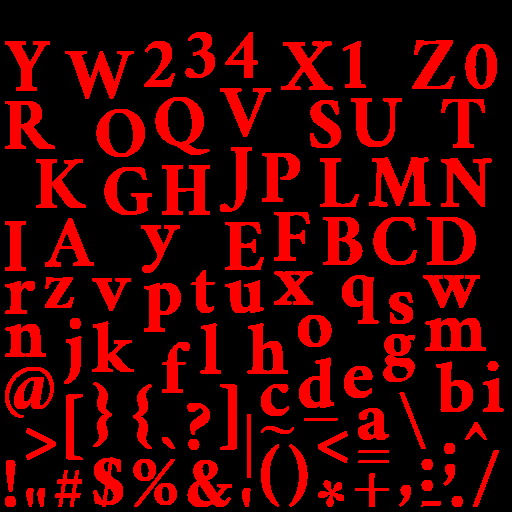
\includegraphics[scale=0.8]{images/font-atlas}
  \caption{Exemple de font atlas en police 72}
  \label{fig:atlas}
\end{figure}

Désormais, nous avons uniquement besoin de changer de texture courante quand on change de font face. C'est parfait puisqu'en moyenne nous utilisons pas plus de deux font à la fois.

Il y a tout de même un prix à payer pour l'utilisation de la texture atlas et celui-ci s'est fait sur la mémoire. En effet il faut maintenant rajouter un attribut à chacun de nos vertices
pour stocker la coordonnée de texture (U,V) afin de définir la sous région dans la texture correspondant au glyphe. Pour résumer, nos vertices contiennent la position, calculée à partir de
la métrique de la glyphe et la texcoord pour plaquer la bonne sous région de la texture atlas.

\subsubsection{Implémentation}

Les fameux rectangles de chaque glyphe sont en réalité composé de deux triangles car la primitive de dessin rectangle n'existe pas. Il faut donc 6 vertices pour afficher un seul caractère.
Nous aurions pu indexer les vertices pour n'afficher un rectangle qu'avec 4 vertices mais nous n'avons pas eu le temps.

Mais que devient donc la couleur ? La couleur n'est effectivement pas stockée dans les vertices, c'est une redondance qui pèserait un poids non négligeable en mémoire. La couleur est une variable
commune à beaucoup de caractères. Nous avons décidé d'envoyer aux shaders la couleur du texte avec une variable dite \og uniform \fg{}, sorte de variable globale, de ce fait il n'y a pas de redondance.
Cette même économie de mémoire pourrait nous être reprochée de casser le batching. C'est vrai que si la couleur la change comme avec les textures, il faut mettre à jour la variable de la couleur
dans le shader. Mais généralement un texte lisible est de couleur uni. De plus, la couleur s'applique à une chaîne de caractères entière et non au caractère. Nous sommes convaincus que nos utilisateurs
n'essaieront pas d'afficher un texte bariolé des couleurs de l'arc-en-ciel, qui de toute façon, pour voir le jour, devrait contenir une marque texte pour chaque caractère de cet artistique texte.
Comme nous venons de le dire plus haut, la couleur s'applique à une marque texte entière, c'est une situation qui ne devrait pas arriver.

Pour en revenir sur l'implémentation dans \textit{contrast}, une marque texte contient uniquement la position, la couleur, le contenu du texte et pour finir une référence (sous forme
de chaîne de caractères). Toutes les fonts faces (FaceCache) sont stockés dans un cache (FontCache) contenu dans \textit{contrast}. Elles sont indexées dans un tableau associatif (HashMap) avec la référence
comme clef. C'est pour éviter tout problème mémoire lié à Rust. Ainsi, quand \textit{contrast} fabrique les vertices des marques textes, il a juste à récupérer la clef correspondant à la font face,
vérifier si elle est présente, et procéder. Accessoirement, cela permet à l'utilisateur de changer la taille de police d'une font, il suffit qu'il enregistre un nouveau couple font et police
sous une autre clef et il pourra s'en servir.

Nous n'allons pas détailler le shader de cette marque, il n'utilise pas de géometrie shader, fonction de distance ou autre sucrerie.
Il ne represente pas la partie intéressante de l'implémentation. Il ne mérite donc pas que nous nous y attardions.

\subsubsection{Petites subtilitées}

Il faut savoir que lorsque FreeType rastérise un glyphe, le bitmap qu'il produit a son axe Y inversé par rapport à celui de \textit{contrast}. Par défaut donc, les glyphes sont dessinés la tête en bas.
Ce n'est pas pratique à lire vous en conviendrez. Pour ne pas compliquer les calculs de nos shaders, nous avons décidé d'inverser directement les bitmaps produits avant de les envoyer
dans la texture atlas.

À noter, il n'existe pas de glyphe pour le caractère espace. Par conséquent l'espace est simplement un déplacement de la taille de l'advance d'un point d'exclamation.

\subsection{Les calques}
\subsubsection{Qu'est-ce qu'un calque ?}
Un calque est un groupe de marques ayant en commun une profondeur. C'est-à-dire que les marques étant dans
un calque de profondeur 0 apparaîtront devant des marques appartenant à un calque de profondeur 1.

\begin{figure}[htp]
  \centering
  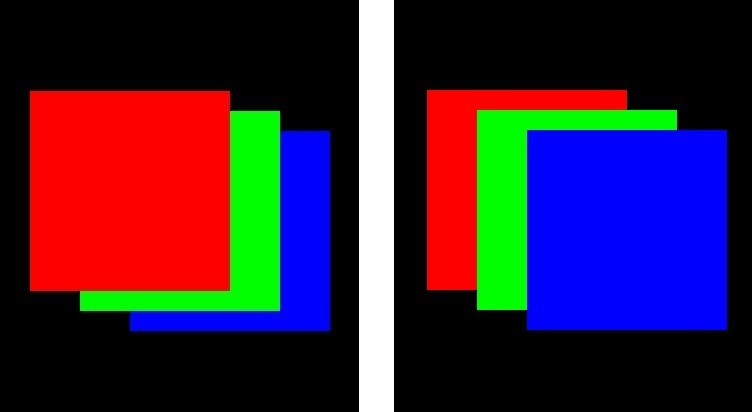
\includegraphics[scale=0.8]{images/calque-exemple}
  \caption{Exemple d'application des calques}
  \label{fig:calque-ex}
\end{figure}

Le code ayant produit les marques de la deuxième image est décrit au listing ~\ref{lst:code-calque}.

\begin{listing}[H]
    \caption{Morceau de code illustrant l'utilisateur des calques}
    \begin{minted}[bgcolor=back, tabsize=4, fontfamily=courier, fontsize=\small, xleftmargin=5pt, xrightmargin=5pt]{rust}

    [...]
    contrast.set_current_layer(2);

    contrast.add_point_mark()
        .set_position((pos.x + 230.0, pos.y, 0.0))
        .set_size((200.0, 200.0))
        .set_color(Color::red())
        .set_shape(Shape::Rectangle)
        .get_id();

    contrast.set_current_layer(1);

    contrast.add_point_mark()
        .set_position((pos.x + 270.0, pos.y + 20.0, 0.0))
        .set_size((200.0, 200.0))
        .set_color(Color::green())
        .set_shape(Shape::Rectangle)
        .get_id();

    contrast.set_current_layer(0);

    contrast.add_point_mark()
        .set_position((pos.x + 310.0, pos.y + 40.0, 0.0))
        .set_size((200.0, 200.0))
        .set_color(Color::blue())
        .set_shape(Shape::Rectangle)
        .get_id();

    [...]
    \end{minted}
    \label{lst:code-calque}
\end{listing}

La figure~\ref{fig:calque-ex} représente deux captures d'écran de marques.
Ces marques ont la même position et la même couleur dans les deux cas, mais nous avons échangé le calque
de la marque rouge avec celui de la marque bleue dans la deuxième capture, mettant ainsi la marque bleue
au premier plan.

\subsubsection{Implémentation}

Tout d'abord, nous avons besoin d'une collection pour stocker les marques de notre calque.
Nous avons choisi de les stocker dans un vecteur pour plusieurs raisons.
La \href{https://doc.rust-lang.org/std/collections/index.html}{documentation} de Rust précise que le
vecteur et la hashmap sont à utiliser dans la plupart des cas et que ces deux collections sont très
performantes.
De plus, nous souhaitons pouvoir être capable de récupérer une marque en O(1) et ajouter une marque en
O(1) (bien que l'ajout n'est pas dans tous les cas en temps constant, par exemple dans le cas où le
vecteur a besoin d'être réalloué pour augmenter sa taille). Ces contraintes nous confortent dans notre
choix du vecteur.

Nous n'avons pas mentionné la suppression des marques volontairement. La raison est que nous ne supprimons
jamais de marques de nos vecteurs. La motivation derrière ce choix est que nous souhaitons une performance
maximale, ce qui implique avoir l'ajout, la récupération et la suppression en temps constant, quitte à
ce que la consommation mémoire soit importante.
Ainsi, nous avons introduit un mécanisme d'invalidation de marques. Lorsque l'utilisateur souhaitera
supprimer une marque et ne plus l'afficher dans sa fenêtre, \textit{contrast} invalidera la marque.
L'invalidation d'une marque indique à \textit{contrast} qu'il faudra l'ignorer lors du prochain
rafraichissement de l'écran, la faisant ainsi disparaître de la fenêtre.

Ce mécanisme seul n'est pas très intelligent car nous pourrions très vite accumuler des marques invalides
, qui ne servent à rien, dans notre vecteur.
C'est pour cette raison que nous avons introduit une pile stockant les index des marques invalides.
La pile nous permet un ajout en O(1) et c'est tout ce dont nous avons besoin pour stocker nos index.
Désormais, lors de la suppression d'une marque, nous empilons également l'index de cette marque.
Lors de l'ajout d'une marque, nous pouvons dépiler, si notre pile n'est pas vide, pour remplacer la
marque invalide à cet index par une nouvelle marque valide.

Ce mécanisme, bien que performant, complexifie légèrement l'ajout de nouvelle marque. Il ne suffit pas de
push une marque dans le vecteur, il faut d'abord vérifier s'il y a des marques invalides qui peuvent être
remplacées.
De plus, une marque ne pouvant pas être dans deux calques à la fois, lorsque l'on souhaite ajouter une
marque dans un calque et que celle-ci était déjà dans un autre calque, il faut nécessairement :
\begin{itemize}
\item cloner la marque de l'ancien calque
\item invalider la marque de l'ancien calque
\item ajouter correctement le clone de la marque dans le nouveau calque
\end{itemize}
Pour cloner la marque, le nouveau calque a besoin de connaître les autres calques. C'est pourquoi un
calque a un pointeur vers \textit{contrast}. Cela permet à un calque d'accéder aux autres calques et d'en
récupérer les  marques. C'est également la raison pour laquelle le code des calques contient une zone
\gls{unsafe}. Nous avons besoin de déréférencer le pointeur de \textit{contrast} pour accéder aux calques et à
leurs marques.

Nous avons également ajouté deux fonctions utilitaires permettant d'appliquer des modifications à toutes
les marques d'un calque. L'une permet de faire bouger les marques d'une certaine distance, l'autre prend
en paramètre une fonction définie par l'utilisateur, et applique cette fonction aux marques. L'utilisateur
peut ainsi appliquer n'importe quelle modification à l'ensemble des marques d'un calque.

\subsection{Animation des marques}
\subsubsection{Qu'est-ce qu'une animation de marque ?}

Une marque animée est une marque dont le changement de propriété se fait progressivement.
Si l'on change la position d'une marque animée, on verra la marque se déplacer de manière fluide vers la
nouvelle position. Si l'on change la forme d'un marque de type point, nous verrons la transformation en la nouvelle forme progressivement.
La figure~\ref{fig:anim-ex} illustre la transformation d'une marque ayant la forme \og Astérisque \fg{} vers une
forme \og Trèfle \fg{}.

\begin{figure}[htp]
  \centering
  
\includegraphics[scale=0.8]{images/anim-exemple}
  \caption{Exemple d'animation pour le changement de forme}
  \label{fig:anim-ex}
\end{figure}

\subsubsection{Implémentation}

Par manque de temps, nous n'avons pas implémenté les animations en utilisant 3 buffers, comme c'était le
cas pour FATuM. Cela nous aurait demandé un changement trop important de l'architecture déjà en place.

À la place, nous avons créé une structure avec un type générique, \textit{AnimationAttribute}.
Notre structure de marque doit contenir autant d'\textit{AnimationAttribute} qu'il y a de propriétés et le
type paramamétré sera celui de la propriété.
Cette structure permet de stocker :
\begin{itemize}
\item La valeur de l'attribut qu'avait la marque avant le début de l'animation, que nous appelerons l'\og
\textit{ancienne valeur} \fg{}.
\item La valeur qu'aura l'attribut de la marque à la fin de l'animation, la \og \textit{valeur cible} \fg{}
\item Le temps au moment où l'animation a commencé, le \og \textit{temps de début} \fg{}.
\end{itemize}

Pour effectuer une animation d'une propriété, nous utilisons la fonction
\textit{\href{https://www.khronos.org/registry/OpenGL-Refpages/gl4/html/mix.xhtml}{mix}} de GLSL, qui effectue une
interpolation linéaire entre deux valeurs.
Elle prend 3 paramètres :
\begin{itemize}
\item le début de la plage dans laquelle interpoler, \og \textit{x} \fg{}
\item la fin de la plage dans laquelle interpoler, \og \textit{y} \fg{}
\item la valeur à utiliser pour interpoler entre x et y, \og \textit{a} \fg{}.
\end{itemize}

\textit{x} correspond à l'\textit{ancienne valeur} de la propriété et \textit{y} correspond à la
\textit{valeur cible}.
Pour obtenir une animation propre et fluide, il faudrait que \textit{a} croisse lentement de 0 à 1.
Pour revenir à l'exemple d'animation de forme précédent, 0 correspondrait à la première marque, 0.5
correspondrait à la troisième, et 1 correspondrait à la dernière.

Le \textit{temps de début} est récupéré grâce à un timer que nous lançons au démarrage du programme.
En passant ce timer aux shaders en tant qu'\gls{uniform}, nous sommes donc capable d'obtenir une croissance
de \textit{a} nous garantissant une animation fluide, en utilisant la formule suivante :
\textit{valeur interpolée = mix(ancienne valeur , valeur cible , min(t - temps de début , 1.0))} où t est
le temps  écoulé depuis le lancement de l'application.
Nous utilisons la fonction minimum pour s'assurer que \textit{a} se dépasse jamais 1. Une valeur de
\textit{a} supérieure à 1 donne lieu à des formes très étranges et fausse.

Jusqu'ici, les animations fonctionnent. Seulement, rien n'empêche l'utilisateur de modifier une propriété pendant une animation, donnant lieu à des comportements confus.
Pour cette raison, nous ignorons les modifications faites à une propriété si celle-ci est en cours
d'animation.

On notera également que cette implémentation permet d'animer plusieurs propriétés en même temps.

\subsubsection{Difficultés rencontrées}

La première difficulté a été de trouver comment implémenter les animations sans modifier l'architecture
principale. La solution a été de modifier directement les structures des
marques en elles-mêmes et de ne pas toucher à la structure principale. La partie précédente décrit plus en
détails l'implémentation de cette solution.

La deuxième difficulté a été d'implémenter les animations dans \textit{contrast}.
En effet, dans un premier temps, nous les avions implémenté de manière indépendante à \textit{contrast} et avec une seule marque. Cette implémentation marchait certes correctement mais l'adapter à \textit{contrast} n'a pas été trivial.
Dans cette implémentation, nous détections la fin d'une animation de manière différente. Nous vérifions
dans la boucle principale si l'animation était terminée pour chaque marque, et nous la mettions à jour si
c'était le cas.
Mais imaginons cette mécanique avec plus de 200 000 marques : si elles étaient toutes animées en même
temps, l'application ne pourrait jamais atteindre les 60 images par seconde.
Nous avons donc enlevé cette vérification quand nous avons implémenté les animations dans \textit{contrast}
pour des raisons évidentes de performances.
À la place, nous vérifions si une animation est finie seulement lorsque que l'on souhaite modifier la
marque, donc dans les setters.

\subsection{Les actions liées aux touches}

\subsubsection{Implémentation}

Dans la partie haut niveau de \textit{contrast}, nous avons donné la possibilité à
l’utilisateur de lier des touches du clavier qu’il aura choisi à des actions.

La boucle de rendu principal de \textit{luminance} s'occupe pour nous d'écouter les
évènements utilisateurs : pression de touche, clic de souris, etc.
Cependant, l'utilisateur n'a pas accès à cette boucle. Nous avons donc ajouté des
fonctions permettant, à l'appui d'une touche choisie par l'utilisateur, d'exécuter une
fonction elle aussi définie par l'utilisateur.

Les signatures des fonctions que l'utilisateur peut lier aux touches sont cependant
décidées par la bibliothèque. Nous en avons fournit trois :
\begin{itemize}
\item une fonction prenant en paramètre seulement la touche qui déclenchera l'action.
Cette fonction permet principalement de récupérer des marques ou des calques pour
afficher leurs propriétés
\item une fonction prenant en paramètre la touche et un identifiant de marque. Celle-ci
permet d'appliquer des modifications en temps réelle à la marque représentée par cet
identifiant.
\item une fonction prenant en paramètre la touche et une liste d'identifiants, permettant de modifier les marques représentées par ces derniers.
\end{itemize}

Les fonctions qui seront définies par l'utilisateur sont stockées dans une union de fonction appelée \textit{Callback}.

Nous pouvons stocker des fonctions avec des signatures différentes mais
comment les lier à des touches ?
La solution la plus évidente est d'utiliser une hashmap avec la touche du clavier comme clé et un \textit{Callback} comme valeur.

Nous sommes capable à présent, dans la boucle principale du renderer, de vérifier, quand
une touche a été appuyée, si elle était liée à un \textit{Callback}. Si c'est le cas,
nous appelons simplement la fonction correspondante.

\subsubsection{Difficultés rencontrées}

Les paramètres sur lesquels influent l'utilisateur sont donc limités car ces fonctions
doivent obligatoirement respectées les signatures définies par la bibliothèque.
Une bonne solution aurait été d'utiliser des closures (ou fonctions anonymes). De cette
manière, l'utilisateur aurait été beaucoup plus libre pour écrire ses actions.

On pourrait représenter cette solution avec une syntaxe de ce type
(voir listing~\ref{lst:ex-closure}).
\begin{listing}[H]
    \caption{Exemple d'un lien touche/action avec l'utilisation d'une closure}
    \begin{minted}[bgcolor=back, tabsize=4, fontfamily=courier, fontsize=\small, xleftmargin=5pt, xrightmargin=5pt]{rust}
    [...]
    let contrast = renderer.get_contrast_mut();
    [...]
    renderer.add_action_on_press(Key::A, || {
        // code de la closure
    }
    \end{minted}
    \label{lst:ex-closure}
\end{listing}

Le problème apparaît si l'utilisateur utilise la variable \textit{contrast} dans la
closure. Le comportement des closures fait qu'elle sera capturée et empruntée
mutablement une seconde fois (la première fois étant lors de la déclaration de la
variable \textit{contrast}). Hors comme précédemment indiqué, on ne peut emprunter une
variable qu'une seule fois.

C'est la raison pour laquelle nous avons opté pour l'approche décrite en début de
partie.

\subsection{Les identifiants de marques}

L'utilisateur manipule des marques. Mais pour retrouver une marque existante et y
appliquer des modifications, nous avons besoin de son identifiant.

La structure représentant un identifiant de marque comprend toutes les données dont nous
avons besoin pour retrouver une marque, c'est-à-dire l'index du calque où elle est
stockée et l'index de la marque en elle-même dans le conteneur de marques du calque.
Que se passe t-il alors lorsque l'on ajoute une marque qui était déjà dans un calque à
un autre calque ? L'identifiant auquel a accès l'utilisateur deviendra faux car les index
auront changés.

Nous devons alors, à chaque modification d'une marque, mettre à jour le réel
identifiant de la marque mais également l'identifiant auquel a accès l'utilisateur, qui n'est pas le même.
Effectivement, si l'utilisateur avait accès au réel identifiant, le problème ne se
poserait pas.

Il y avait deux méthodes qui aurait permis d'avoir accès au réel identifiant :
\begin{itemize}
\item en utilisant des pointeurs : la méthode \textit{get\_id()} renverrait un pointeur
vers le véritable identifiant et le problème serait résolu. Cependant, il y avait un gros
inconvénient à cette méthode, que nous avons rencontré quand nous avons tenté
d'implémenter cette solution : à chaque fois que devions déréférencer ce pointeur, nous
devions mettre le code dans une zone non sûre. Cela générait beaucoup de zones non sûres
et nous faisait dévier de l'un des principes de Rust qui est de faire du code sûr. Nous
avons donc décider d'abandonner
cette idée.
\item en utilisant une référence : une référence étant grossièrement, en Rust, un
pointeur safe, nous pourrions résoudre le problème. La méthode \textit{get\_id()}
retournerait ainsi une référence pointant vers le réel identifiant.

En utilisant un concept de Rust, nous nous heurtons à un autre problème lié à Rust :
l'ownership. Le but ici n'étant pas d'expliquer tous les paradigmes de Rust, nous
définirons simplement l'ownership en disant que c'est le moyen qu'utilise Rust pour gérer la mémoire.

Récupérer une référence signifie que l'on emprunte l'objet vers lequel la référence
pointe. L'objet en question étant dans un conteneur qui lui-même appartient à une
structure (la structure principale), emprunter cet objet revient à emprunter toute la
structure.

Nous pouvons emprunter plusieurs fois la structure tant que nous faisons des
emprunts immutables, c'est-à-dire que nous promettons à Rust de ne jamais modifier cette
structure. Nous ne pouvons cependant emprunter mutablement qu'une seule fois dans un scope, empêchant donc l'utilisateur de modifier les marques comme il le souhaite.
Cette idée a donc elle aussi était mis de côté.
\end{itemize}

Notre solution est donc que \textit{get\_id()} renvoie une copie du réel identifiant. A chaque
fois que l'utilisateur souhaite modifier une marque, il doit passer une référence mutable
de la copie dont il dispose pour que nous puissions la mettre à jour en même temps que
le réel identifiant.

\subsection{Bibliothèques externes utilisées}
\subsubsection{lazy\_static}
Nous utilisons cette bibliothèque \cite{lazy-static} une seule fois dans
\textit{contrast} : pour déclarer le timer. Nous avons besoin qu'il soit valide pendant
toute la durée du programme et nous voulons qu'il soit accessible partout dans le code.
C'est ce que cette bibliothèque permet de faire : déclarer facilement des variables
statiques en Rust.

\subsubsection{rand}
C'est une bibliothèque \cite{rand} permettant de générer des nombres aléatoirement. Nous
l'utilisons dans le but de fournir une fonction permettant de retourner une forme
aléatoire.

\subsubsection{nalgebra}
Nous utilisons cette bibliothèque \cite{nalgebra} uniquement pour calculer une matrice de projection orthographique.
C'est le coeur de notre caméra 2D. C'est un calcul tout de même fastidieux alors nous considérons cette bibliothèque totalement justifiée.

\subsubsection{freetype-rs et rect-packer}
Ces deux bibliothèques sont indispensable pour implémenter la marque texte et nous l'avons expliqué pourquoi dans la section qui lui est dédié.

\section{Analyse du fonctionnement du logiciel}

\subsection{Ce qui fonctionne}

\subsection{Ce qui ne fonctionne pas}

\subsection{Tests et résultats}

Nous avons intensivement testé la structure principale, \textit{contrast}, ainsi que toutes ses méthodes.
L'ajout de marque dans les calques et le système d'invalidation des marques ont également subi beaucoup de tests.

Le test sur l'invalidation des marques est particulièrement intéressant : nous créons
une structure \textit{contrast}, à laquelle nous ajoutons et enlevons des éléments
successivement. Nous créons ensuite une autre structure \textit{contrast}, à laquelle
nous rajoutons manuellement les marques que la première structure était censée contenir,
la validité des marques, etc.
Nous comparons ensuite ces deux structures. Le but est qu'elles soient parfaitement identique.

Les structures de données des marques ont peu voir aucun test car leur comportement
est plutôt trivial.

\subsection{Les bugs}

A notre connaissance, il n'y a pas de bugs dans notre implémentation.

Cependant, le comportement des calques n'est pas vraiment celui souhaité.
Nos calques ont la capacité de comporter plusieurs type de marques mais ils ne
fonctionneront pas correctement. C'est-à-dire qu'une marque point à la couche 0 (qui
doit être tout devant) pourra se retrouver derrière une marque ligne qui est à la couche 1.
La raison pour cela est que nous affichons les marques type par type puis calque par
calque.
Les  calques marchent cependant correctement s'ils comportent seulement des marques du même type.

\section{Conclusion}

Nous avons réussi le coeur de notre bibliothèque ainsi que certaines fonctionnalités
secondaires.

Il y a cependant des éléments manquants et extensions possibles.
Voici une liste non-exhaustive :

\begin{itemize}
\item Les marques aires. La structure pour les stocker serait la même que pour les
polygones mais leurs shaders seraient différents
\item Différents modes de dessin pour les lignes : en tirets, pointillets, fléchées
\item La gestion des polygones sécants
\item Les animations pour toutes les marques. Actuellement, seulement les marques points
sont animées
\item La technique qu'utilise FATuM pour les animations, le triple buffering
\item Des calques pouvant gérer plusieurs types de marques.
\end{itemize}

%\nocite{*}
\printglossaries
\printbibliography

\end{document}
